\documentclass[11pt]{article}
\usepackage{amsfonts}
\usepackage{amsmath}
\usepackage{amsthm}
\usepackage{amssymb}
\usepackage{mathrsfs}
\usepackage[fit]{truncate}
\usepackage{acl2012}
\usepackage{times}
\usepackage{latexsym}
\usepackage{amsmath}
\usepackage{url}
\usepackage{graphicx}
\usepackage{caption}
\usepackage{multirow}
\usepackage{dblfloatfix}
\usepackage{float}
\usepackage{subfigure}
\DeclareMathOperator*{\argmax}{arg\,max}
\setlength\titlebox{5cm}    % Expanding the titlebox

\newcommand{\affliationPenn}{\ensuremath{{}^\text{1}}}
\newcommand{\affliationJHU}{\ensuremath{{}^\text{2}}}

\title{A large scale study of the languages spoken (by bilinguals) on Mechanical Turk}
\title{The Language Demographics of  Amazon Mechanical Turk}

\author{Ellie Pavlick\affliationPenn \ \ \ \ \ Ann Irvine\affliationJHU  \ \ \ \ \ Dmitry Kachaev\affliationJHU  \ \ \ \ \  Chris Callison-Burch\affliationPenn$^{,}$\affliationJHU \\
\affliationPenn Computer and Information Science Department, University of Pennsylvania \\
\affliationJHU Human Language Technology Center of Excellence, Johns Hopkins University \\
  }
  
% Anonymized for submission
\author{}

\date{}

\begin{document}
\maketitle

\begin{abstract}
We present a large scale study of the languages spoken by bilingual workers on Mechanical Turk (MTurk).  
We establish a  methodology for determining the language skills of anonymous crowd workers that is more robust than simple surveying.  We validate workers' self-reported language skill claims by measuring their ability to correctly translate words, and by geolocating workers to see if they reside in countries where the languages are likely to be spoken. Rather than posting a one-off survey, we posted paid tasks consisting of 1,000 assignments to translate a total of 10,000 words in each of 119 languages.  Our study ran for several weeks, and was highly visible on the MTurk crowdsourcing platform, increasing the chances that bilingual workers would complete it.  Our study was useful both to create bilingual dictionaries and to act as census of the bilingual speakers on MTurk.  We use this data to recommend languages with the largest speaker populations as good candidates for other researchers who want to  develop crowdsourced, multilingual technologies.

\end{abstract}

\section{Overview}
Crowdsourcing is a promising new mechanism for collecting data for natural language processing research. Access to a fast, cheap, and flexible workforce allows us to collect new types of data, potentially enabling new language technologies.
Because crowdsourcing platforms like Amazon Mechanical Turk (MTurk) give researchers access to a worldwide workforce, one obvious application of crowdsourcing is the creation of multilingual technologies. 
With an increasing number of active crowd workers located outside of the United States, there is even the potential to reach fluent speakers of lower resource languages.
In this paper, we investigate the feasibility of hiring language informants on MTurk by conducting the first large-scale demographic study of the languages spoken by workers on the platform. 

There are several complicating factors when trying to take a census of workers on MTurk.  The workers' identities are anonymized, and Amazon provides no information about their countries of origin or their language abilities.  Posting a simple survey to have workers report this information may be inadequate, since (a) many workers may never see the survey, (b) many opt not to do one-off surveys since potential payment is low, and (c) validating the answers of respondents is not straightforward. 

Our study establishes a methodology for determining the language demographics of anonymous crowd workers that is more robust than simple surveying. We ask workers what languages they speak and what country they live in, and validate their claims by measuring their ability to correctly translate words and by recording their geolocation.  To increase the visibility and the desirability of our tasks, we post 1,000 assignments in each of 119 languages.  These tasks each consist of translating 10 foreign words into English.  Two of the 10 words have known translations, allowing us to validate that the workers' translations are accurate.  We construct bilingual dictionaries with up to 10,000 entries, with the majority of entries being new. 

Surveying thousands of workers allows us to analyze current speaker populations for more than 100 languages.  The data also allows us to answer questions like: 
How quickly is work completed in a given language? 
Are crowdsourced translations reliably good? 
How often do workers misrepresent their language abilities to obtain financial rewards? 

%%%%%%%%%%%%%%% MAP OF WORKER LOCATIONS %%%%%%%%%%%
\begin{figure*}[h]
\centering
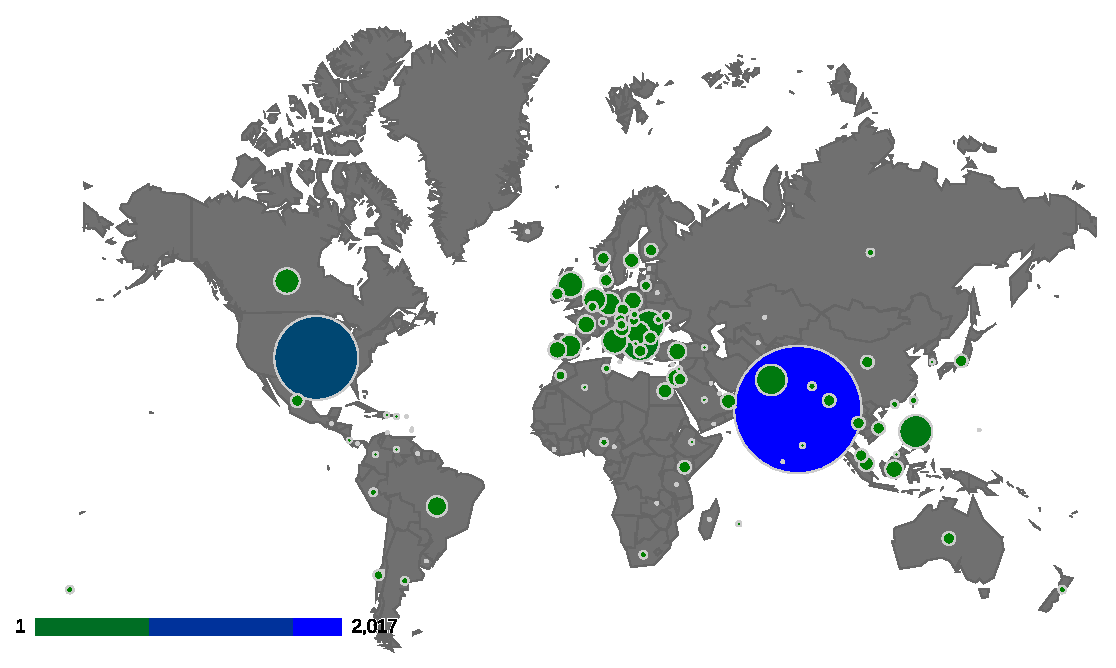
\includegraphics[width=\linewidth]{final-figures/turkermap}
\caption{The number of workers per country.  This map was generated based on geolocating the IP address of  5,277 workers in our study.  The size of the circles represents the number of workers from each country.  The two largest are India (2,017 workers) and the United States (904).  To calibrate the sizes: the Philippines has 147 workers, Egypt has 25, Russia has 10, and Sri Lanka has 4.}
\label{map}
\end{figure*}
%%%%%%%%%%%%%%%%%%%%%%%%%%%%%%%%%%%%%%%

\section{Background and Related Work}
Amazon's Mechanical Turk (MTurk) is an online marketplace for work that gives employers and researchers access to a large, low-cost, workforce. MTurk allows employers to provide micro-payments in return for workers completing micro-tasks.  The basic units of work on MTurk are called `Human Intelligence Tasks' (HITs).  MTurk was designed to accommodate tasks that are difficult for computers, but simple for people. This facilitates research into human computation, where people can be treated as a function call \cite{vonAhnThesis,Little2009,quinn-bederson:2011}.  It has application to research areas like human-computer interaction \cite{bigham-et-al:2010,bernstein-et-al:2010}, computer vision  \cite{sorkin-forsyth:2008,deng-et-al:2010,rashtchian:10}, speech processing \cite{marge:10,lane-EtAl:2010:MTURK,Parent-Eskenazi:2011,Eskenazi:2013:crowdsourcing-speech-book},  and natural language processing \cite{Snow2008,callisonburch-dredze:2010:MTURK,laws-scheible-schutze:2011:EMNLP}. 

\nocite{novotney-callisonburch:2010:NAACLHLT}

On MTurk, researchers who need work completed are called `Requesters', and workers are often referred to as `Turkers'.  MTurk is a true market, meaning that Turkers are free to choose to complete the HITs which interest them, and Requesters can price their tasks competitively to try to attract workers and have their tasks done quickly \cite{faridani-et-al:2011,singer-mittal:2011}. Turkers remain anonymous to Requesters, \nocite{Lease2013}
and all payment occurs through Amazon. Requesters are able to accept submitted work or reject work that does not meet their standards.  Turkers are only paid if a Requester accepts their work. 

Several reports examine Mechanical Turk as an economic market \cite{ipeirotis:2010:marketplace,lehdonvirta-ernkvist:2011}.  When Amazon introduced MTurk, it first offered payment only in Amazon credits, and later offered direct payment in US dollars. More recently, it has expanded to include one foreign currency, the Indian rupee. Despite its payments being limited to two currencies or Amazon credits, MTurk claims over half a million workers from 190 countries \cite{AmazonRequesterTour}.  This suggests that its worker population should represent a diverse set of languages.

A demographic study by \newcite{ipeirotis:2010:demographics} focused on age, gender, martial status, income levels, motivation for working on MTurk, and whether workers used it as a primary or supplemental form of income.  The study contrasted Indian and US workers. \newcite{Ross2010} completed a longitudinal follow-on study. 
A number of other studies have informally investigated Turkers' language abilities.  \newcite{munro-tily:2011} compiled survey responses of 2,000 Turkers, revealing that four of the six most represented languages come from India (the top six being Hindi, Malayalam, Tamil, Spanish, French, and Telugu).  \newcite{irvine:10} had Turkers evaluate the accuracy of translations that had been automatically inducted from monolingual texts.  They examined translations of 100 words in 42 low-resource languages, and reported geolocated countries for their workers (India, the US, Romania, Pakistan, Macedonia, Latvia, Bangladesh and the Philippines).  Irvine and Klementiev discussed the difficulty of quality control and assessing the plausibility of workers' language skills for rare languages, which we address in this paper. 

Several researchers have investigated using MTurk to build bilingual parallel corpora for machine translation, a task which stands to benefit low cost, high volume  translation on demand \cite{Germann2001}.  \newcite{ambati_act} conducted a pilot study by posting 25 sentences to MTurk for Spanish, Chinese, Hindi, Telugu, Urdu, and Haitian Creole.  In a study of 2000 Urdu sentences, 
\newcite{zaidan-callisonburch:2011:ACL-HLT2011a} presented methods for achieving professional-level translation quality from Turkers by soliciting multiple English translations of each foreign sentence. 
\newcite{Zbib-etal:2012:NAACL} used crowdsourcing to construct a 1.5 million word parallel corpus of dialect Arabic and English, training a statistical machine translation system that produced higher quality translations of dialect Arabic than a system a trained on 100 times more Modern Standard Arabic-English parallel data.  \newcite{post-callisonburch-osborne:2012:WMT} used MTurk to build parallel corpora between English and six Indian languages, ranging from .5M to 1.5M words, and use them to demonstrate the efficacy of syntactic machine translation on verb-final languages.  
Several researchers have examined cost optimization using active learning techniques to select the most useful sentences or fragments to translate \cite{ambati_naacl,bloodgood-callisonburch:2010:ACL,AmbatiThesis}.

To contrast our research with previous work, the main contributions of this paper are: (1) a robust methodology for assessing the bilingual  skills of anonymous workers, (2) the largest-scale census to date of language skills of workers on MTurk, and (3) a detailed analysis of the data gathered in our study.

%%%%%%%%%%%%%%% NAT LANG PIE TABLE %%%%%%%%%%%
\begin{table}
\footnotesize
\begin{tabular}{lrlrlr}\hline\hline
%Language&\# Turkers\\
\hline
English&592&	French&63&	Vietnamese&34\\
Tamil&253&	Polish&61&	Macedonian&31\\
Malayalam&219&	Urdu&56&	Cebuano&29\\
Hindi&149&	Tagalog&54&	Swedish&26\\
Spanish&131&	Marathi&48&	Bulgarian&25\\
Telugu&87&	Russian&44&	Hungarian&23\\
Chinese&86&	Italian&43&	Swahili&23\\
Romanian&85&	Bengali&41&	Thai&22\\
Portuguese&82&	Gujarati&39&	Catalan&22\\
Arabic&74&	Hebrew&38&	Lithuanian&21\\
Kannada&72&	Dutch&37&	Punjabi&21\\
German&66&	Turkish&35&	Others &$\leq$20\\
\hline\hline
\end{tabular}
\normalsize
\caption{Self-reported native language of 3,154 bilingual Turkers. Not shown are 54 languages with $\leq$20 speakers. 
We omit 1,797 Turkers who did not report their native language, 243 who reported 2 native languages, and 83 with $\geq$3 native languages.}\label{lang-pie}
\end{table}
%%%%%%%%%%%%%%%%%%%%%%%%%%%%%%%%%%%%%%%

\section{Survey Design}
The central task in this study was to investigate Mechanical Turk's bilingual population.  We accomplished this through self-reported surveys combined with a HIT to translate individual words for over 100 languages.  We evaluate the accuracy of the workers' translations against known translations.  In cases where these were not exact matches, we used a second pass monolingual HIT, which asked English speakers to evaluate if a worker-provided translation was a synonym of the known translation.

\paragraph{Demographic questionnaire}

At the start of each HIT, Turkers were asked to complete a brief survey about their language abilities. The survey asked the following questions:
\begin{itemize}
\item Is [language] your native language? 
\item How many years have you spoken [language]? 
\item Is English your native language? 
\item How many years have you spoken English?
\item What country do you live in?
\end{itemize}
We automatically collected each worker's current location by geolocating their IP address.  A total of 5,277 unique workers completed our HITs.  Among those, 3,890 provided responses to our survey questions, and we were able to geolocate 5,050.  Figure \ref{map} plots the location of workers across 111 countries.  Table \ref{lang-pie} gives the most common self-reported native languages. 

\paragraph{Selection of languages}

We drew our data from the different language versions of Wikipedia.   We selected the 100 languages with the largest number of articles,\footnote{\url{http://meta.wikimedia.org/wiki/List_of_Wikipedias}} and then selected an additional 19 low resource languages, giving a total of 119 languages (Table \ref{wikipedia-buckets}). For each language, we chose the 1,000 most viewed articles over a 1 year period,\footnote{\url{http://dumps.wikimedia.org/other/pagecounts-raw/}} and extracted the 10,000 most frequent words from them. The resulting vocabularies served as the input to our translation HIT.

\begin{table}[h]
\scriptsize 
\begin{center}
\begin{tabular}{|p{0.95\linewidth}|}
\hline
{\sc 500k+ articles:} German (de), English (en), Spanish (es), French (fr), Italian (it), Japanese (ja), Dutch (nl), Polish (pl), Portuguese (pt), Russian (ru)\\
\hline
{\sc 100k-500k articles:} Arabic (ar), Bulgarian (bg), Catalan (ca), Czech (cs), Danish (da), Esperanto (eo), Basque (eu), Persian (fa), Finnish (fi), Hebrew (he), Hindi (hi), Croatian (hr), Hungarian (hu), Indonesian (id), Korean (ko), Lithuanian (lt), Malay (ms), Norwegian (Bokmal) (no), Romanian (ro), Slovak (sk), Slovenian (sl), Serbian (sr), Swedish (sv), Turkish (tr), Ukrainian (uk), Vietnamese (vi), Waray-Waray (war), Chinese (zh)\\
\hline
{\sc 10k-100k articles:}
Afrikaans (af) Amharic (am) Asturian (ast) Azerbaijani (az) Belarusian (be) Bengali (bn) Bishnupriya Manipuri (bpy) Breton (br) Bosnian (bs) Cebuano (ceb) Welsh (cy) Zazaki (diq) Greek (el) West Frisian (fy) Irish (ga) Galician (gl) Gujarati (gu) Haitian (ht) Armenian (hy) Icelandic (is) Javanese (jv) Georgian (ka) Kannada (kn) Kurdish (ku) Luxembourgish (lb) Latvian (lv) Malagasy (mg) Macedonian (mk) Malayalam (ml) Marathi (mr) Neapolitan (nap) Low Saxon (nds) Nepali (ne) Newar / Nepal Bhasa (new) Norwegian (Nynorsk) (nn) Piedmontese (pms) Sicilian (scn) Serbo-Croatian (sh) Albanian (sq) Sundanese (su) Swahili (sw) Tamil (ta) Telugu (te) Thai (th) Tagalog (tl) Urdu (ur) Yoruba (yo)\\ 
\hline
{\sc $<$10k articles:} Central Bicolano (bcl) Tibetan (bo) Ilokano (ilo) Punjabi (pa) Kapampangan (pam) Pashto (ps) Sindhi (sd) Somali (so) Uzbek (uz) Wolof (wo)\\

\hline
\end{tabular}
\end{center}
\normalsize
\caption{A list of the languages that were used in our study, grouped by the number of Wikipedia articles in the language.  Each language's code is given in parentheses.  These language codes are used in other figures throughout this paper.}\label{wikipedia-buckets}
\end{table}%


%%%%%%%%%%%%%%% HITLANG QUALITY BAR %%%%%%%%%%%
\begin{figure*}[h]
\begin{center}
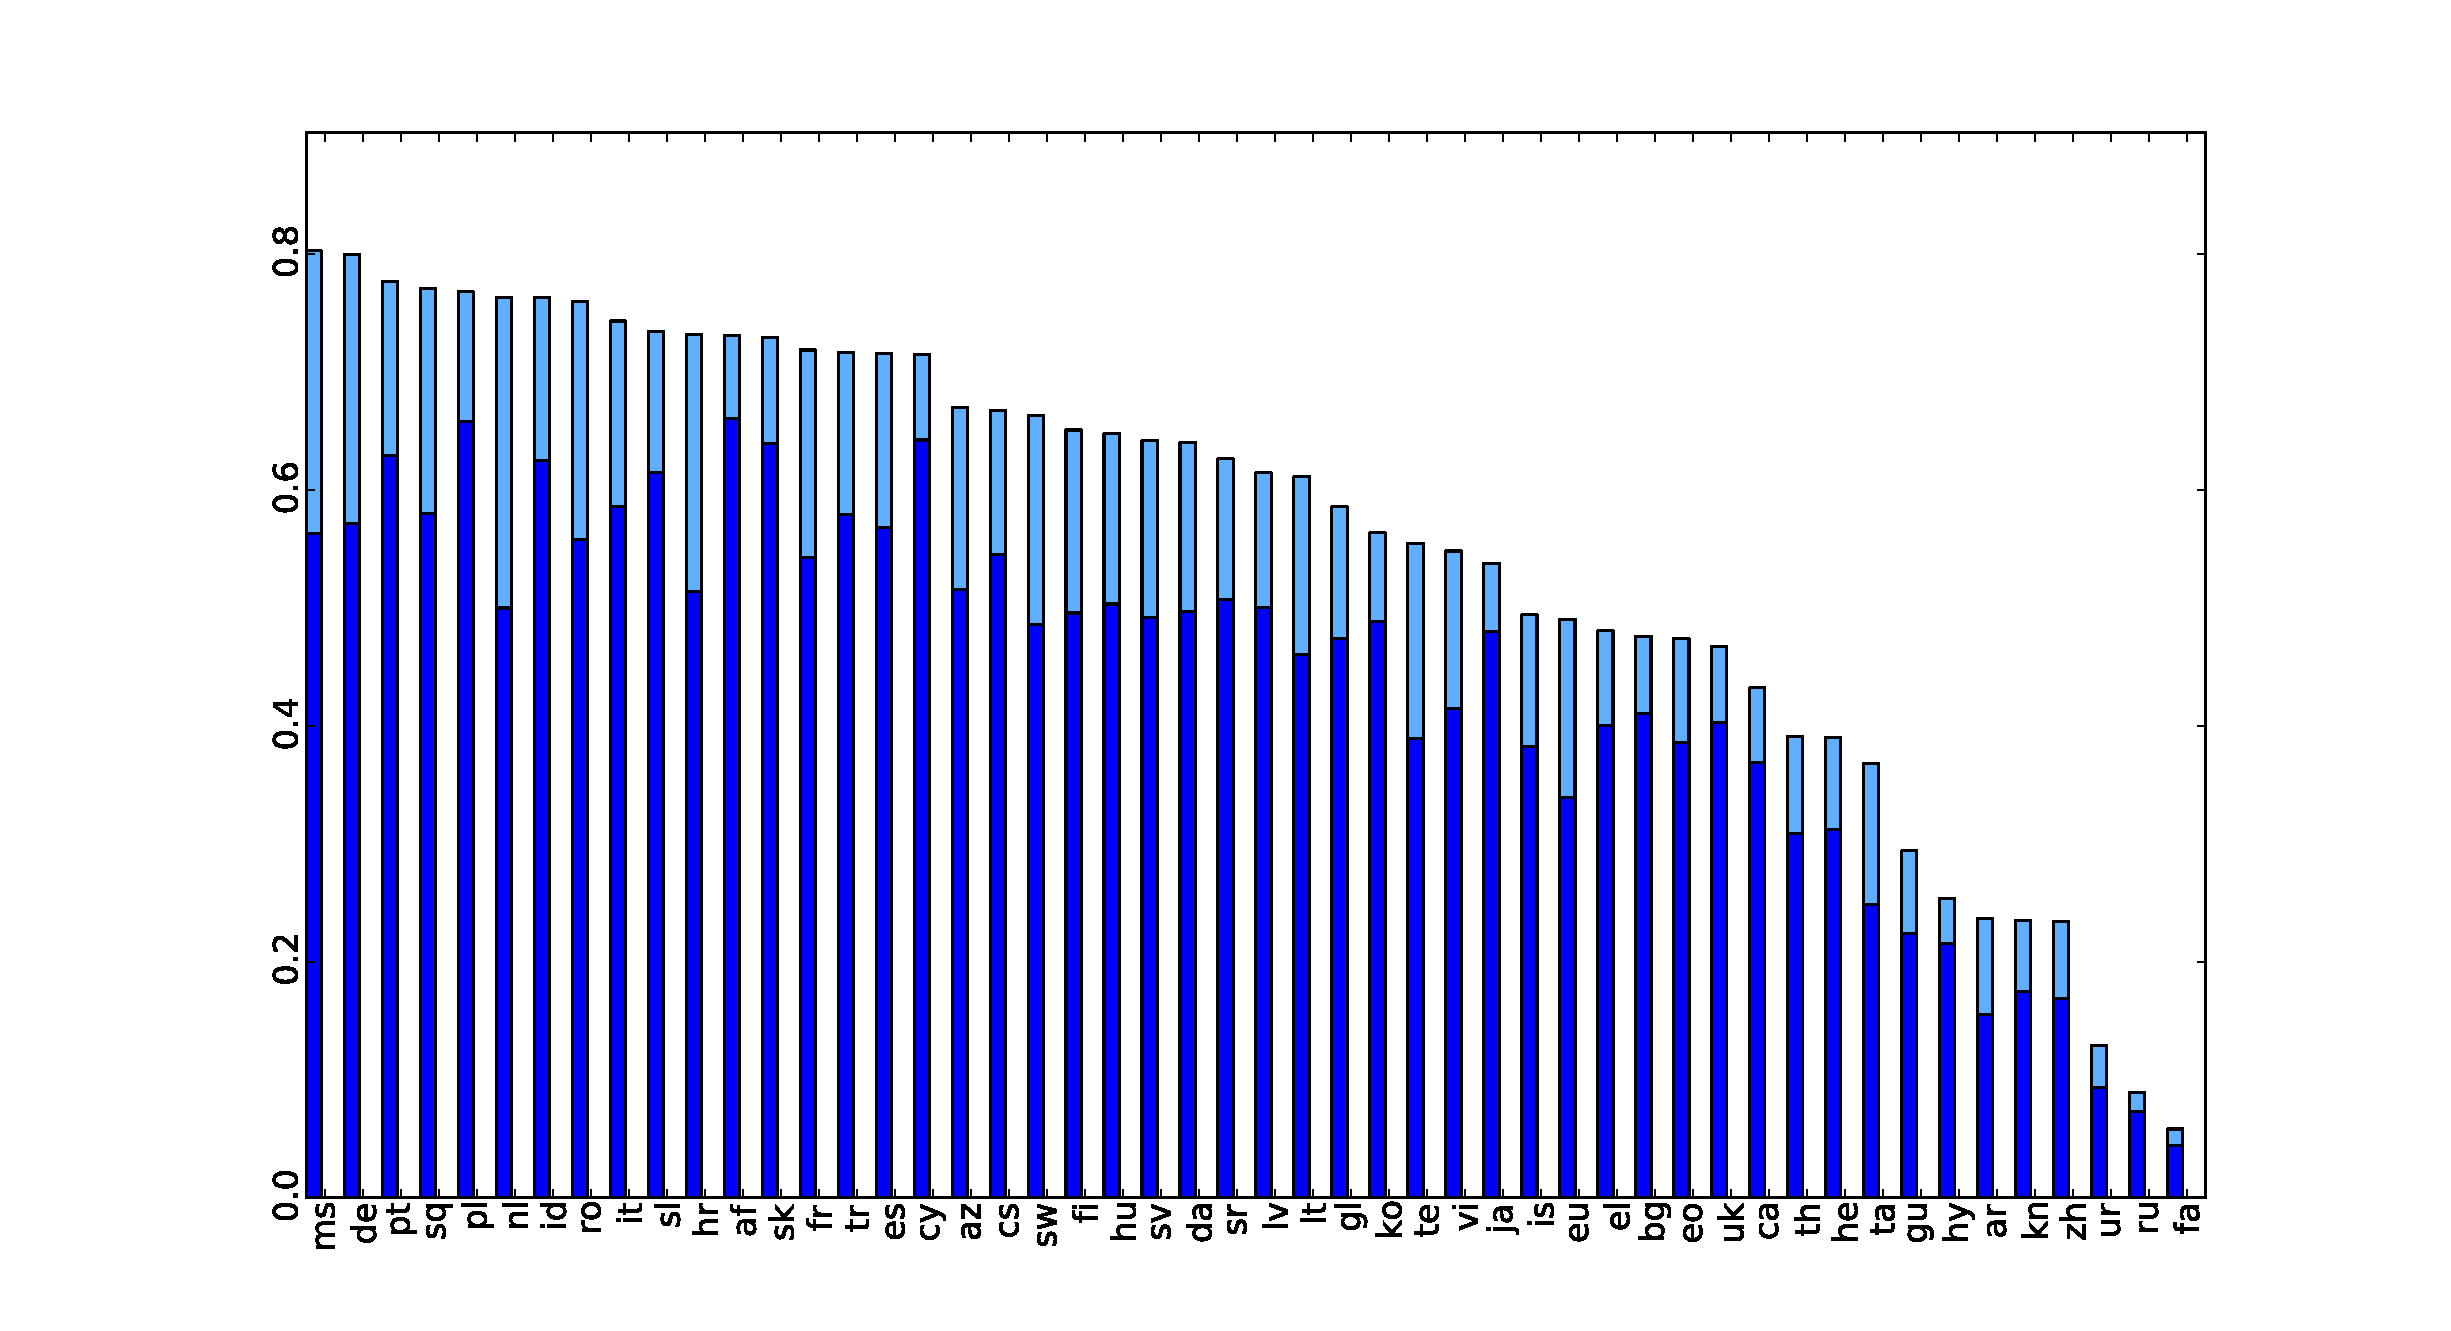
\includegraphics[width=0.8\linewidth]{final-figures/quality-bar}
\caption{Translation quality for languages with at least 50 Turkers.  The dark blue bars indicate the proportion of translations which exactly matched gold standard translations, and light blue indicate translations which were judged to be correct synonyms.}
\label{hitlangqual} 
\end{center}
\end{figure*}
%%%%%%%%%%%%%%%%%%%%%%%%%%%%%%%%%%%%%%%%%%%%%%%%%%%%%%%%



\paragraph{Translation HIT}

For the translation task, we asked Turkers to translate individual words.  We showed each word in the context of three sentences that were drawn from Wikipedia.  
Turkers were allowed to mark that they were unable to translate a word. Each task contained 10 words, 8 of which were words with unknown translations, and 2 of which were quality control words with known translations.   
We gave special instruction for translating names of people and places, giving examples of how to handle `Barack Obama' and `Australia' using their interlanguage links. For languages with non-Latin alphabets, names were transliterated. 

The task paid \$0.15 for the translation of 10 words.  
Each set of 10 words was independently translated by three separate workers.  5,277 workers completed 308,079 translations assignments, totaling more than 3 million words, over a period of three and a half months.

\paragraph{Gold standard translations} 
A set of gold standard translations were automatically harvested from Wikipedia  for every language to use as embedded controls. We used Wikipedia's inter-language links to pair titles of English articles with their corresponding foreign article's title.  To get a more translatable set of pairs, we excluded any pairs where: (1) the English word was not present in the WordNet ontology  \cite{miller1995wordnet}, (2) either article title was longer than a single word, (3) the English wikipedia page was a subcategory of person or place, or (4) the English and the foreign titles were identical or a substring of the other.

\paragraph{Manual evaluation of non-identical translations}
We counted all translations that exactly matched the gold standard translation as correct.  For non-exact matches we created a second-pass quality assurance HIT.  
Turkers were shown a pair of English words, one of which was a Turker's translation of the foreign word used for quality control, and the other of which was the gold-standard translation of the foreign word. Evaluators were asked whether the two words had the same meaning, and chose between three answers: `Yes', `No', or `Related but not synonymous.'  Examples of meaning equivalent pairs include: $<${\it petroglyphs, rock paintings}$>$, $<${\it demo, show}$>$ and  $<${\it loam, loam: soil rich in decaying matter}$>$.  Non-meaning equivalents included: $<${\it assorted, minutes}$>$, and $<${\it major,} URL of image$>$.  Related items were things like $<${\it sky, clouds}$>$. Misspellings like $<${\it lactation, lactiation} $>$ were judged to have same meaning, and were marked as misspelled.   3 separate Turkers judged each pair, allowing majority votes for difficult cases. 


We checked Turkers who were working on this task by embedding pairs of words which were either known to be synonyms (drawn from WordNet) or  unrelated (randomly chosen from a corpus). 
Automating approval/rejections for the second-pass evaluation allowed the whole pipeline to be run automatically.  Caching judgments meant that we ultimately needed only 
20,955 synonym tasks to judge all of the submitted translations (a total of 55,880 unique non-matching word pairs).  These were completed by an additional 1,006 workers.  Each of these assignments included 10 word pairs and paid \$0.10.



\section{Measuring Translation Quality}

We calculate the quality of translations on the level of individual assignments and aggregated over languages and countries.  We define an assignment's quality as the proportion of controls that are correct in a given assignment, where correct means exactly correct or judged to be synonymous or related.
\begin{align}	
	\text{Quality}(a_i) = \frac{1}{k}\sum\limits_{j=1}^{k_i}\mathbf{\delta}(tr_{ij} \in \texttt{syns[$g_j$]})
\end{align}	
where $a_i$ is the $i^{th}$ assignment, $k_i$ is the number of controls in $a_i$, $tr_j$ is the Turker's provided translation of control word $j$ in assignment $i$, $g_j$ is the gold standard translation of control word $j$, \texttt{syns[$g_j$]} is the set of words judged to be synonymous with $g_j$ and includes $g_j$, and $\mathbf{\delta}(x)$ is Kronecker's delta and takes value 1 when $x$ is true. 
Most assignments had two known words embedded, so most assignments had scores of either 0, 0.5, or 1. 

%Since judging overall quality for a language with assignment quality scores is biased towards to small numbers of highly active Turkers, we instead report language quality scores as the average per-Turker quality, where a Turker's quality is  the average quality of all the assignments that she completed:
%\begin{align}	
%	\text{Quality}(t_i) = \frac{\sum_{a_j \in \texttt{assigns[$i$]}\text{Quality}(a_j)}}{\mid \texttt{assigns[$i$]} \mid}
%\end{align}	
%where $t_i$ is the $i^{th}$ Turker, \texttt{assigns[$i$]} is the assignments completed by Turker $i$, and Quality($a$) is as above.
%

Quality for a language is then given by
\begin{align}	
	\text{Quality}(l_i) = \frac{\sum_{a_j \in \texttt{assigns[$i$]}\text{Quality}(a_j)}}{\mid \texttt{assigns[$i$]} \mid}
\end{align}	
where $l_i$ is the ith language, \texttt{assigns[$i$]} is the set of completed assignments for language $i$, and Quality($a$) is as above. Quality for a country is computed the same way.

%Quality for a language is then given by
%\begin{align}	
%	\text{Quality}(l_i) = \frac{\sum_{t_j \in \texttt{Turkers[$i$]}\text{Quality}(t_j)}}{\mid \texttt{Turkers[$i$]} \mid}
%\end{align}	
%where $l_i$ is the ith language, \texttt{Turkers[$i$]} is the set of Turkers who completed assignments for language $i$, and Quality($t$) is as above.


Figure \ref{hitlangqual} shows the translation quality for for languages with contributions from at least 50 workers.  



\section{Data Analysis}

We performed an analysis of our data to address the following questions:
\begin{itemize}
\item How quickly can we expect work to be completed in a particular language? 
\item Do workers accurately represent their language abilities?  Should we constrain tasks by region? 
\item Is the use of machine translation prevalent?  
\item Are our gold standard translations valid? 
%\item What is the quality of crowdsourced translations without quality control versus with it? 
\end{itemize}


\paragraph{Speed of completion}


Figure \ref{completion-time} gives the completion times for 40 languages.  
The 10 languages to finish in the shortest amount of time were: Tamil, Malayalam, Telugu, Hindi, Macedonian, Spanish, Serbian, Romanian, Gujarati, and Marathi. 7 of the 10 fastest languages are from India, which is unsurprising given the geographic distribution of workers.  Some languages follow the pattern of having a smattering of assignments completed early, with the rate picking up later. 

%%%%%%%%%%%%%%% COMPLETION TIME CHART %%%%%%%%%%%
\begin{figure}[h]
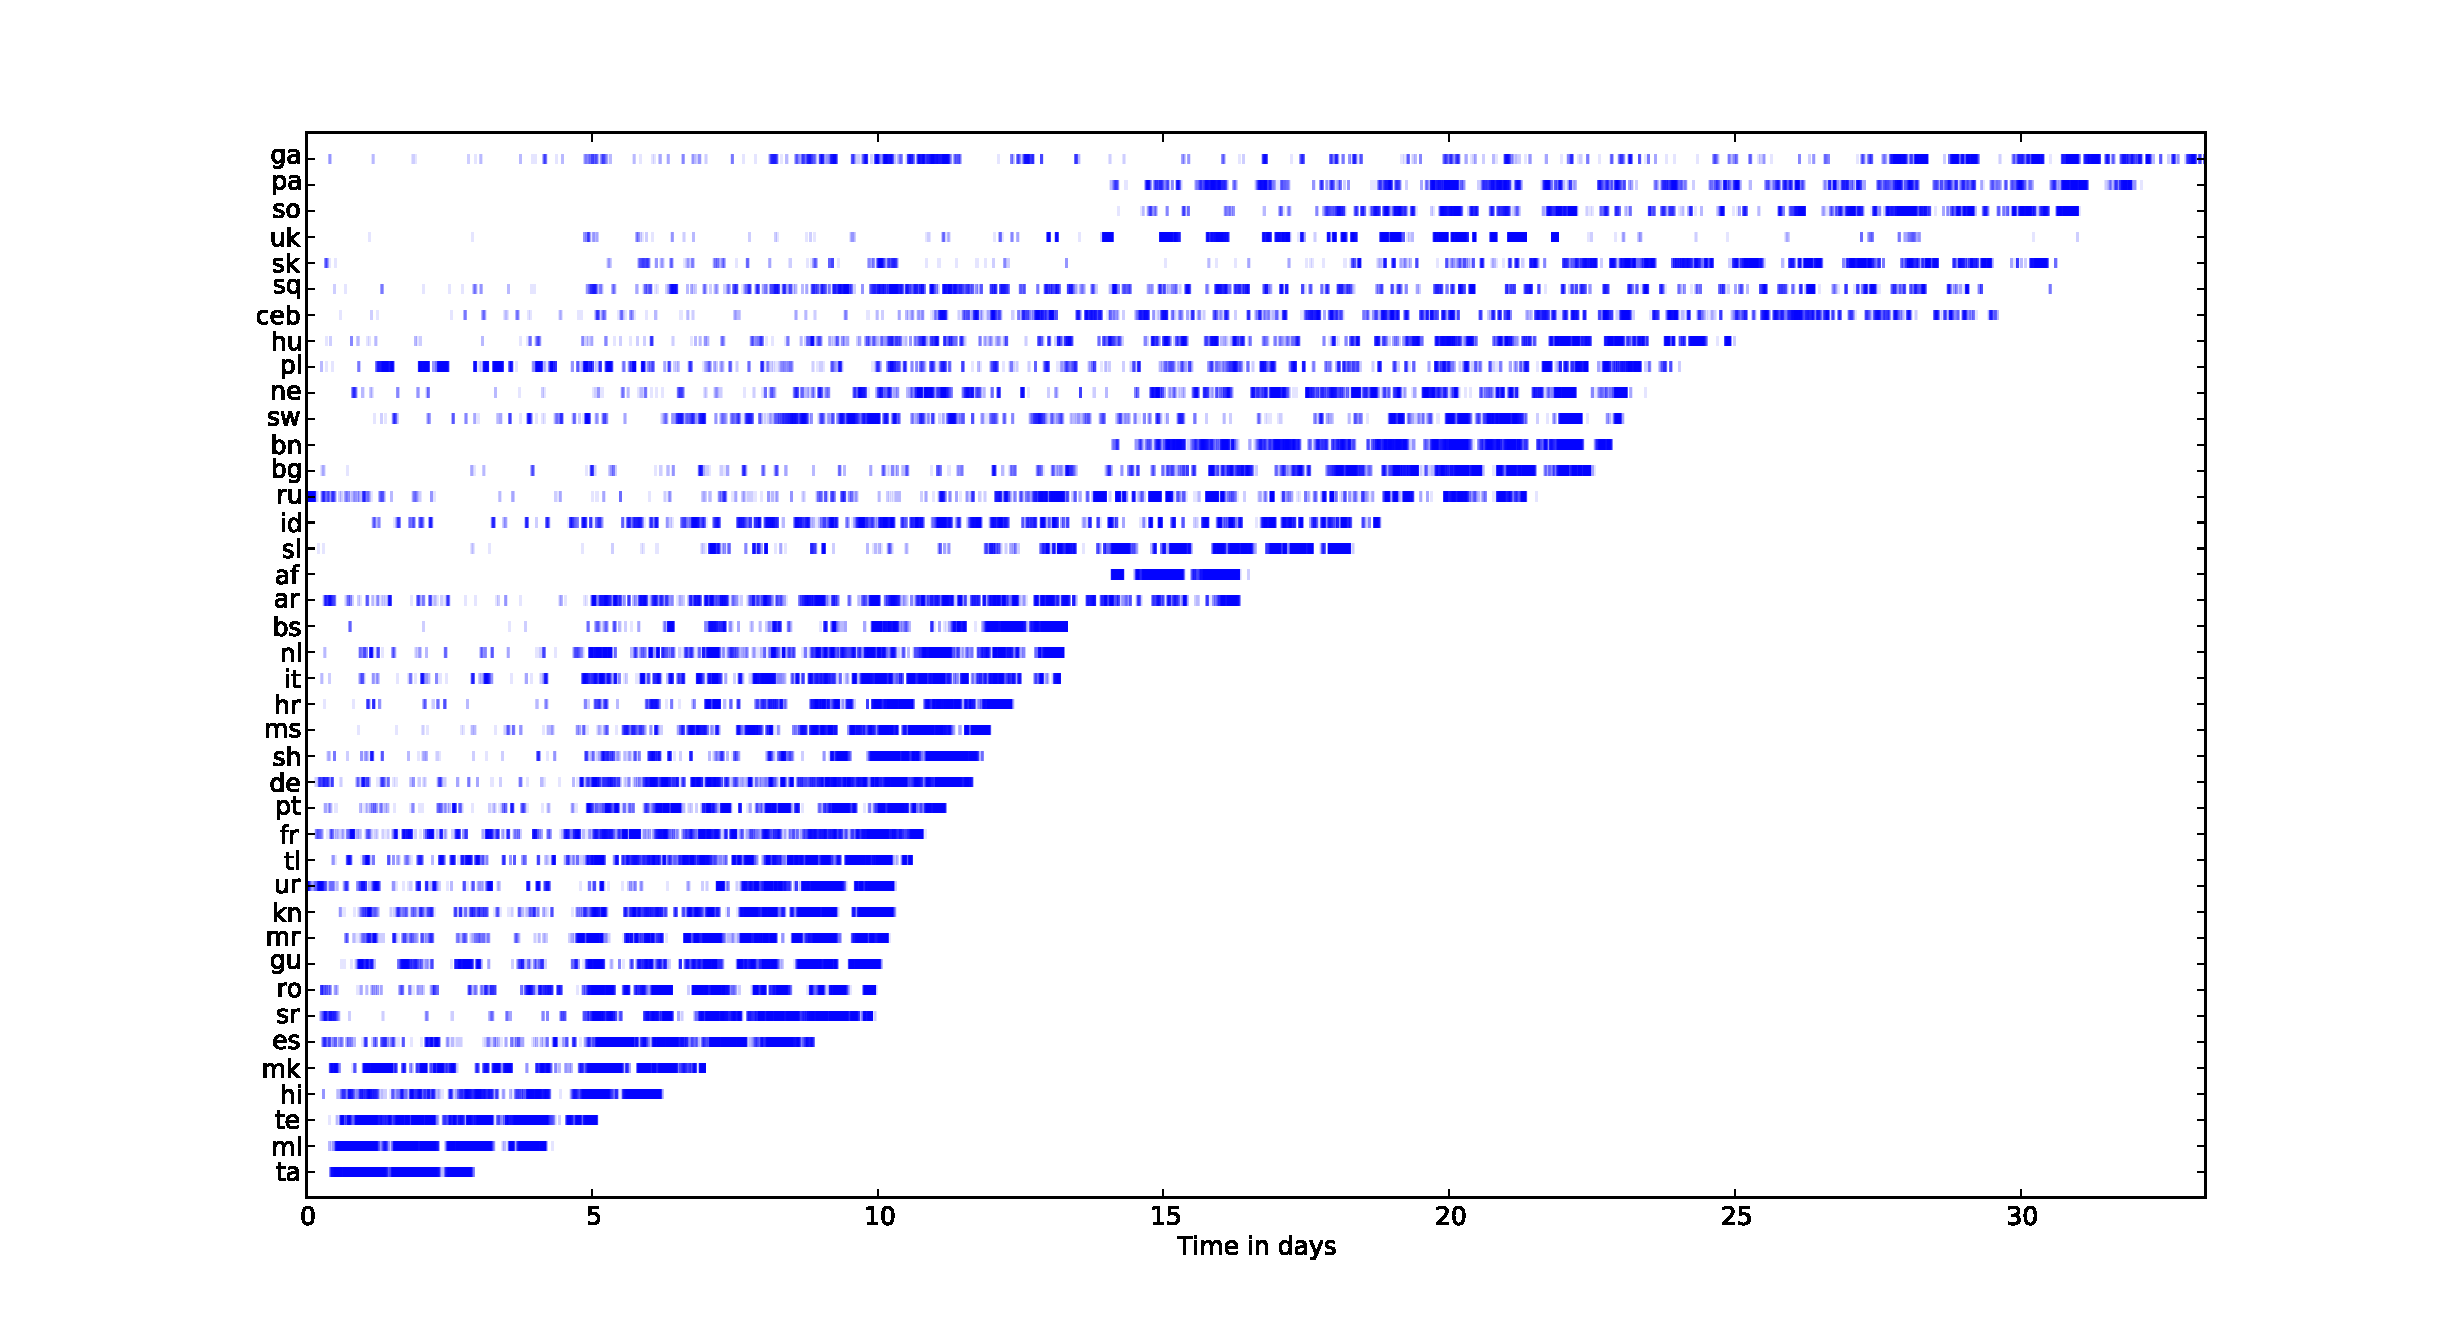
\includegraphics[height=\linewidth,angle=270]{final-figures/completetime}
\caption{Days to complete the translation HITs for 40 of the languages. Tick marks represent the completion of individual assignments. }
\label{completion-time}
\end{figure}
%%%%%%%%%%%%%%%%%%%%%%%%%%%%%%%%%%%%%%%


%%%%%%%%%%%%%%% TURKER QUAL SUMMARY TABLE %%%%%%%%%%%
\begin{table*}
\footnotesize
\begin{tabular}{lllll}
\hline\hline
&\multicolumn{2}{c}{Avg. Turker quality (\# Ts)}&Primary locations&Primary locations\\
&In region&Out of region&of Turkers in region&of Turkers out of region\\
\hline\hline
Hindi&\textbf{0.35} (299)&0.34 (7)&India (285) UAE (5) UK (5) &Saudiarabia (2) Russia (1) Oman (1) \\
Tamil&\textbf{0.37} (278)&0.00 (2)&India (271) US (3) Canada (2) &Tunisia (1) Egypt (1) \\
Malayalam&0.48 (235) &\textbf{0.58} (2)&India (224) UAE (6) US (3) &Saudiarabia (1) Maldives (1) \\
Spanish&\textbf{0.72} (205)&0.61 (23)&US (131) Mexico (18) Spain (14) &India (19) Macedonia (2) Newzealand (1) \\
French&0.65 (183) &\textbf{0.86} (13)&India (68) US (48) France (25) &Greece (3) Japan (2) Netherlands (1) \\
German&\textbf{0.83} (99)&0.65 (58)&Germany (51) US (29) Austria (9) &India (47) Greece (2) UK (2) \\
Italian&\textbf{0.78} (98)&0.71 (51)&Italy (44) US (32) Romania (9) &India (38) Macedonia (2) Ireland (2) \\
Chinese&\textbf{0.24} (121)&0.16 (19)&US (79) Singapore (15) China (14) &Hongkong (6) Australia (3) Germany (2) \\
Malay&0.76 (15) &\textbf{0.83} (110)&Malaysia (8) Singapore (4) US (2) &India (106) Brunei (2) Australia (1) \\
Irish&\textbf{0.68} (58)&0.64 (59)&US (41) Ireland (13) UK (4) &India (45) Macedonia (5) Romania (5) \\
Czech&\textbf{0.71} (52)&0.63 (64)&US (19) Czechrepublic (15) Serbia (5) &Macedonia (30) India (15) UK (5) \\
Turkish&0.72 (83) &\textbf{0.73} (32)&Turkey (39) US (20) Macedonia (12) &India (23) Pakistan (5) Taiwan (1) \\
Amharic&\textbf{0.18} (17)&0.02 (98)&US (14) Ethiopia (3) &India (69) Georgia (9) Macedonia (5) \\
Swedish&\textbf{0.66} (58)&0.61 (56)&US (28) Sweden (23) Finland (3) &India (26) Macedonia (10) Croatia (3) \\
Portuguese&\textbf{0.77} (107)&0.74 (4)&Brazil (46) Portugal (32) US (15) &Pakistan (1) Romania (1) Japan (1) \\
Arabic&0.22 (62) &\textbf{0.26} (48)&Egypt (19) Jordan (17) Morocco (9) &US (20) India (11) Algeria (4) \\
Kannada&\textbf{0.24} (106)&0.00 (1)&India (106) US (1) &France (1) Germany (1) \\
Russian&\textbf{0.09} (72)&0.06 (33)&US (38) Russia (8) Moldova (7) &India (17) Macedonia (4) UK (4) \\
Afrikaans&\textbf{0.74} (4)&0.73 (98)&Southafrica (4) &India (93) Netherlands (2) UAE (1) \\
Sindhi&\textbf{0.15} (93)&0.02 (8)&India (55) Pakistan (37) US (1) &Macedonia (4) Georgia (2) Netherlands (1) \\
\hline\hline
\end{tabular}
\normalsize
\caption{Translation quality when partitioning the translations into two groups, one contains translations submitted by Turkers whose location is within regions that plausibly speak the foreign language, and the other contains translations from Turkers outside those regions.} \label{region-summary}
\end{table*}
%%%%%%%%%%%%%%%%%%%%%%%%%%%%%%%%%%%%%%%%%%%%%%%%%%%%%%%%

\paragraph{Language skills and location}

We measured the average quality of workers who were in countries that plausibly speak a language, versus workers from countries that did not have large speaker populations of that language.  We used the Ethnologue \cite{ethnologue} to compile the list of countries where each language is spoken.  Table \ref{region-summary} compares the average translation quality of assignments completed within the region of each language, and compares it to the quality of assignments completed outside that region. 

Our workers reported speaking 97 languages natively. US workers alone reported 59 native languages. Overall, 4,465 workers were located in a region likely to speak the language from which they were translating, and 3,170 workers were located in countries considered out of region (meaning almost half of our 5,277 Turkers completed HITs in multiple languages). 

Table \ref{region-summary} shows the differences in translation quality when computed using in-region versus out-of-region Turkers, for the languages with the greatest number of workers.  Within region workers typically produced higher quality translations. 
Given the number of Indian workers on Mechanical Turk, it is unsurprising that they represent majority of out-of-region workers.  For the languages that had more than 80 out of region workers (Malay, Amharic, Afrikaans, Icelandic, and Breton), Indian workers represented 90\% of the out of region workers for all of them aside from Amharic.


%When averaged across all languages, there is no significant quality difference between Turkers in region and out of region (0.504 and 0.496, respectively). However, within each language, the effect of location on quality varies greatly (Table \ref{region-summary}). 

% CCB - commented out this figure and paragraph.  I'm not sure that this figure adds any new information
%
%%%%%%%%%%%%%%%% ASSIGNMENT SCATTER %%%%%%%%%%%
%\begin{figure*}[h]
%\centering
%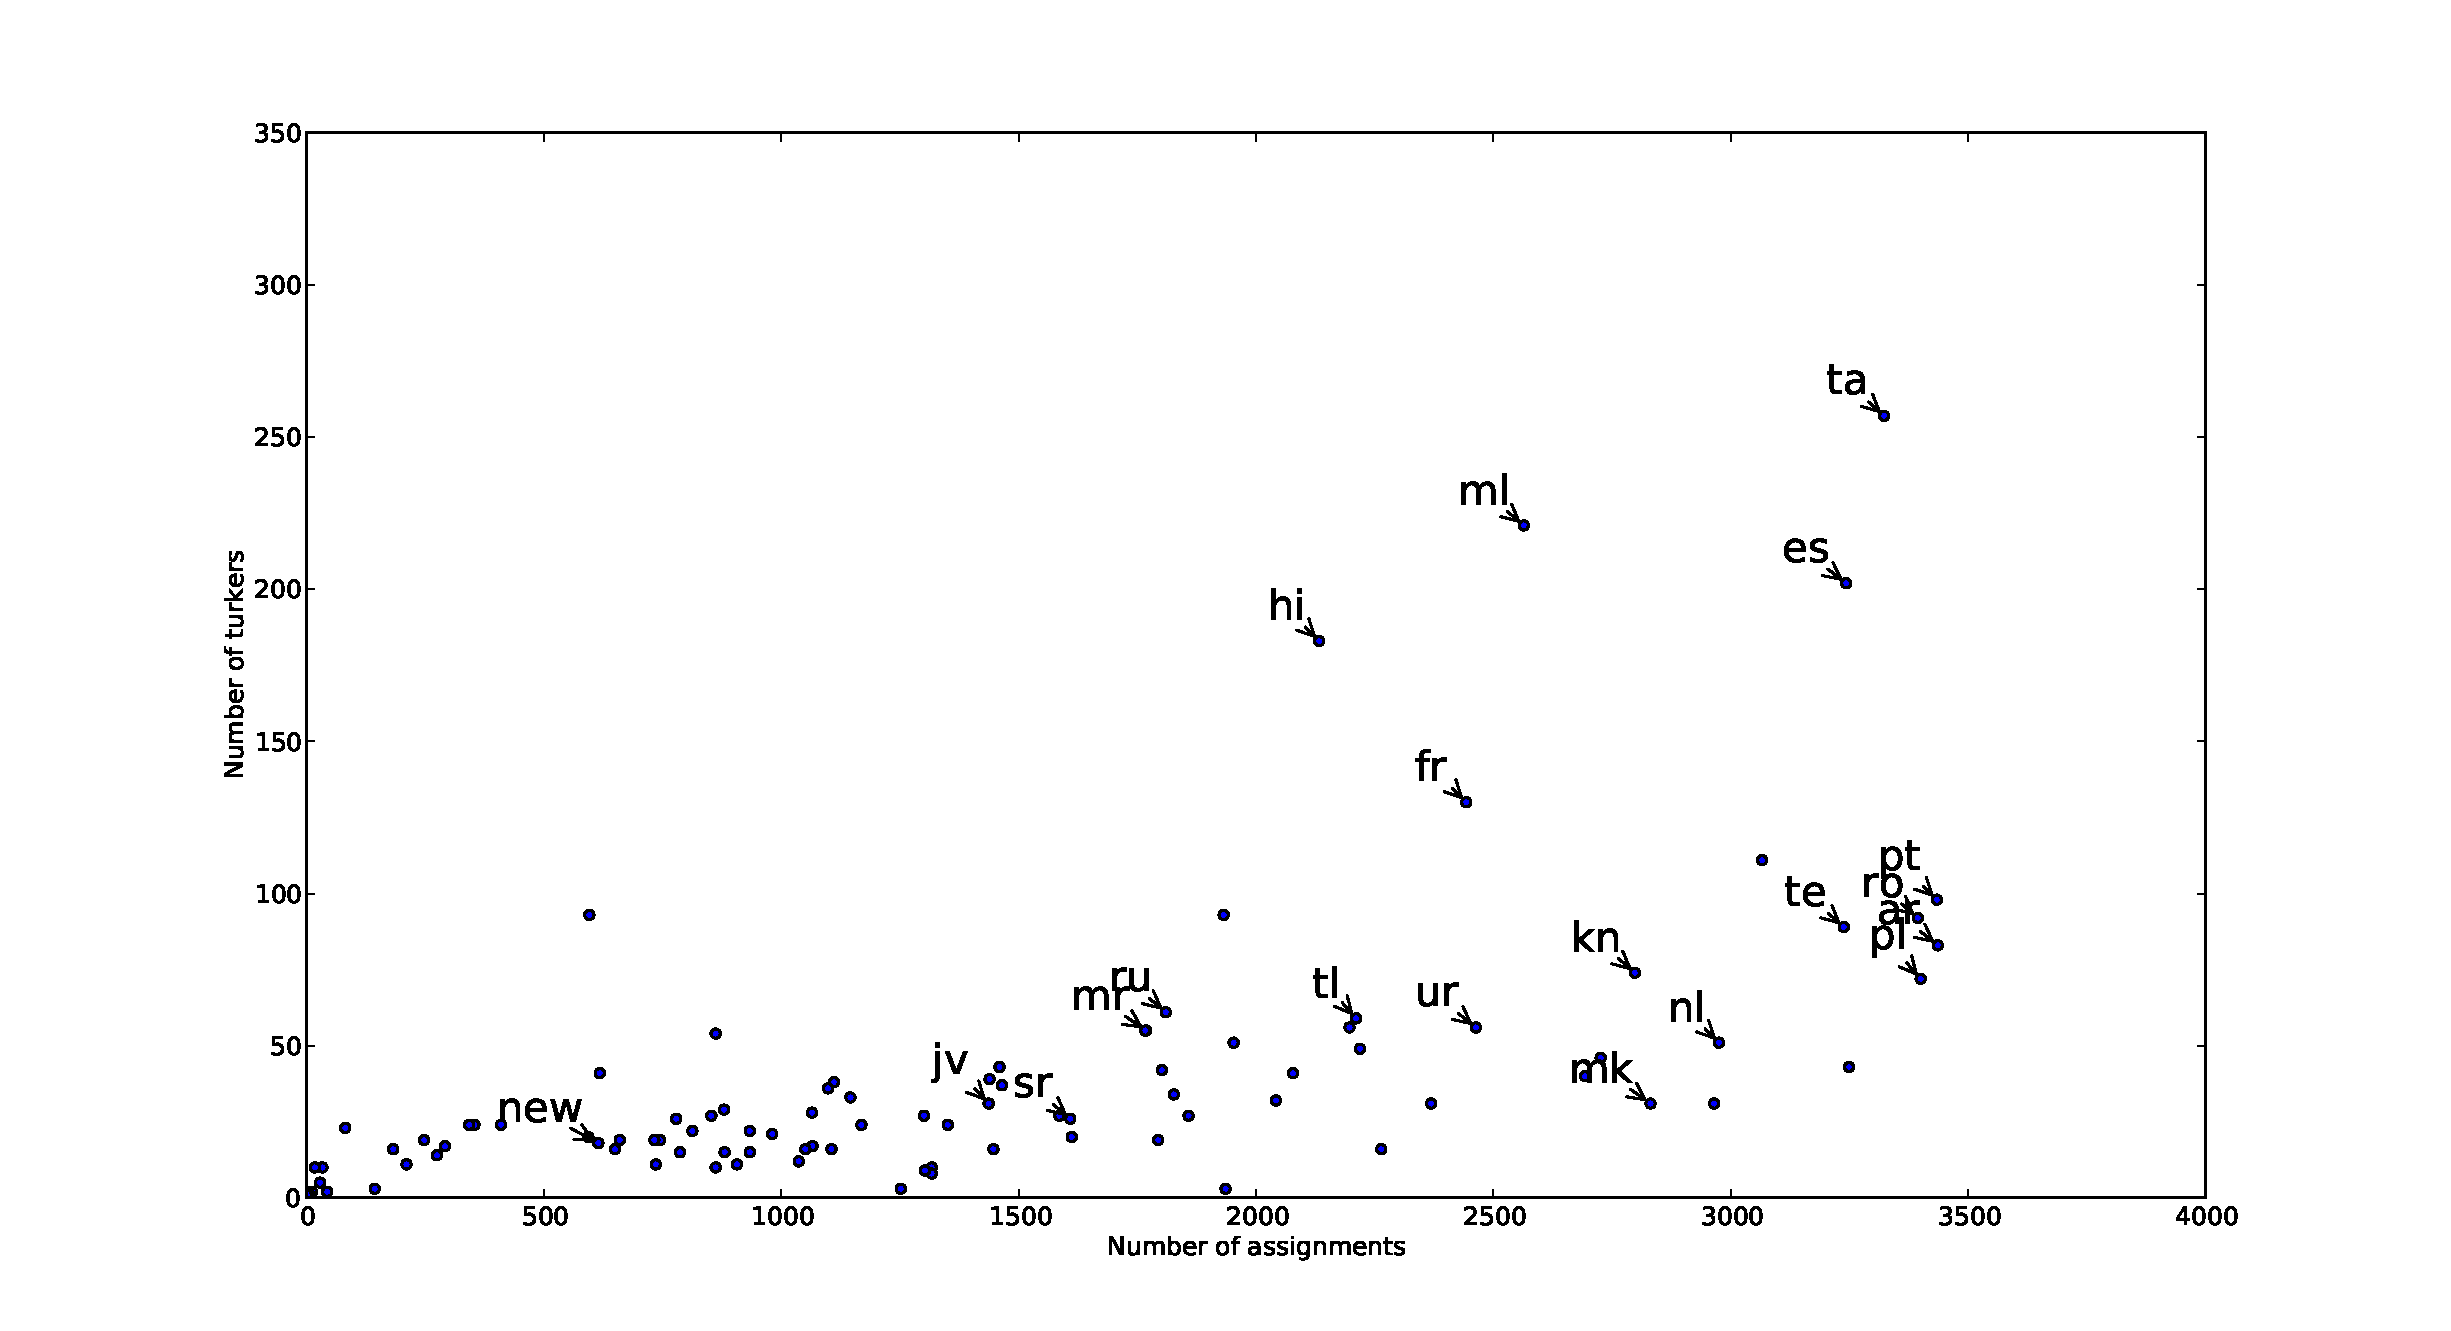
\includegraphics[width=6in]{final-figures/assign-turk-scatter}
%\caption{Number of assignments and number of Turkers for each language. Each dot represents a language. Figure includes only data from Turkers who reported only one native language consistantly across assignments, representing approx. 3900 Turkers across 139,000 assignments.}
%\label{ass-scatter}
%\end{figure*}
%%%%%%%%%%%%%%%%%%%%%%%%%%%%%%%%%%%%%%%%%%%%%%%%%%%%%%%%%
%
%Figure \ref{ass-scatter} shows the volume of HITs completed and the number of workers participating for each language. While the bulk (19\%) of bilingual Turkers report English as their native language (see Figure \ref{lang-pie}), Mechanical Turk's capacity to support the Indian languages is apparent. Hindi, Tamil, and Malayalam are especially well represented in terms of number of active translators. 



%%%%%%%%%%%%%%% HITLANG QUALITY BAR %%%%%%%%%%%
\begin{figure}[h]
\begin{center}
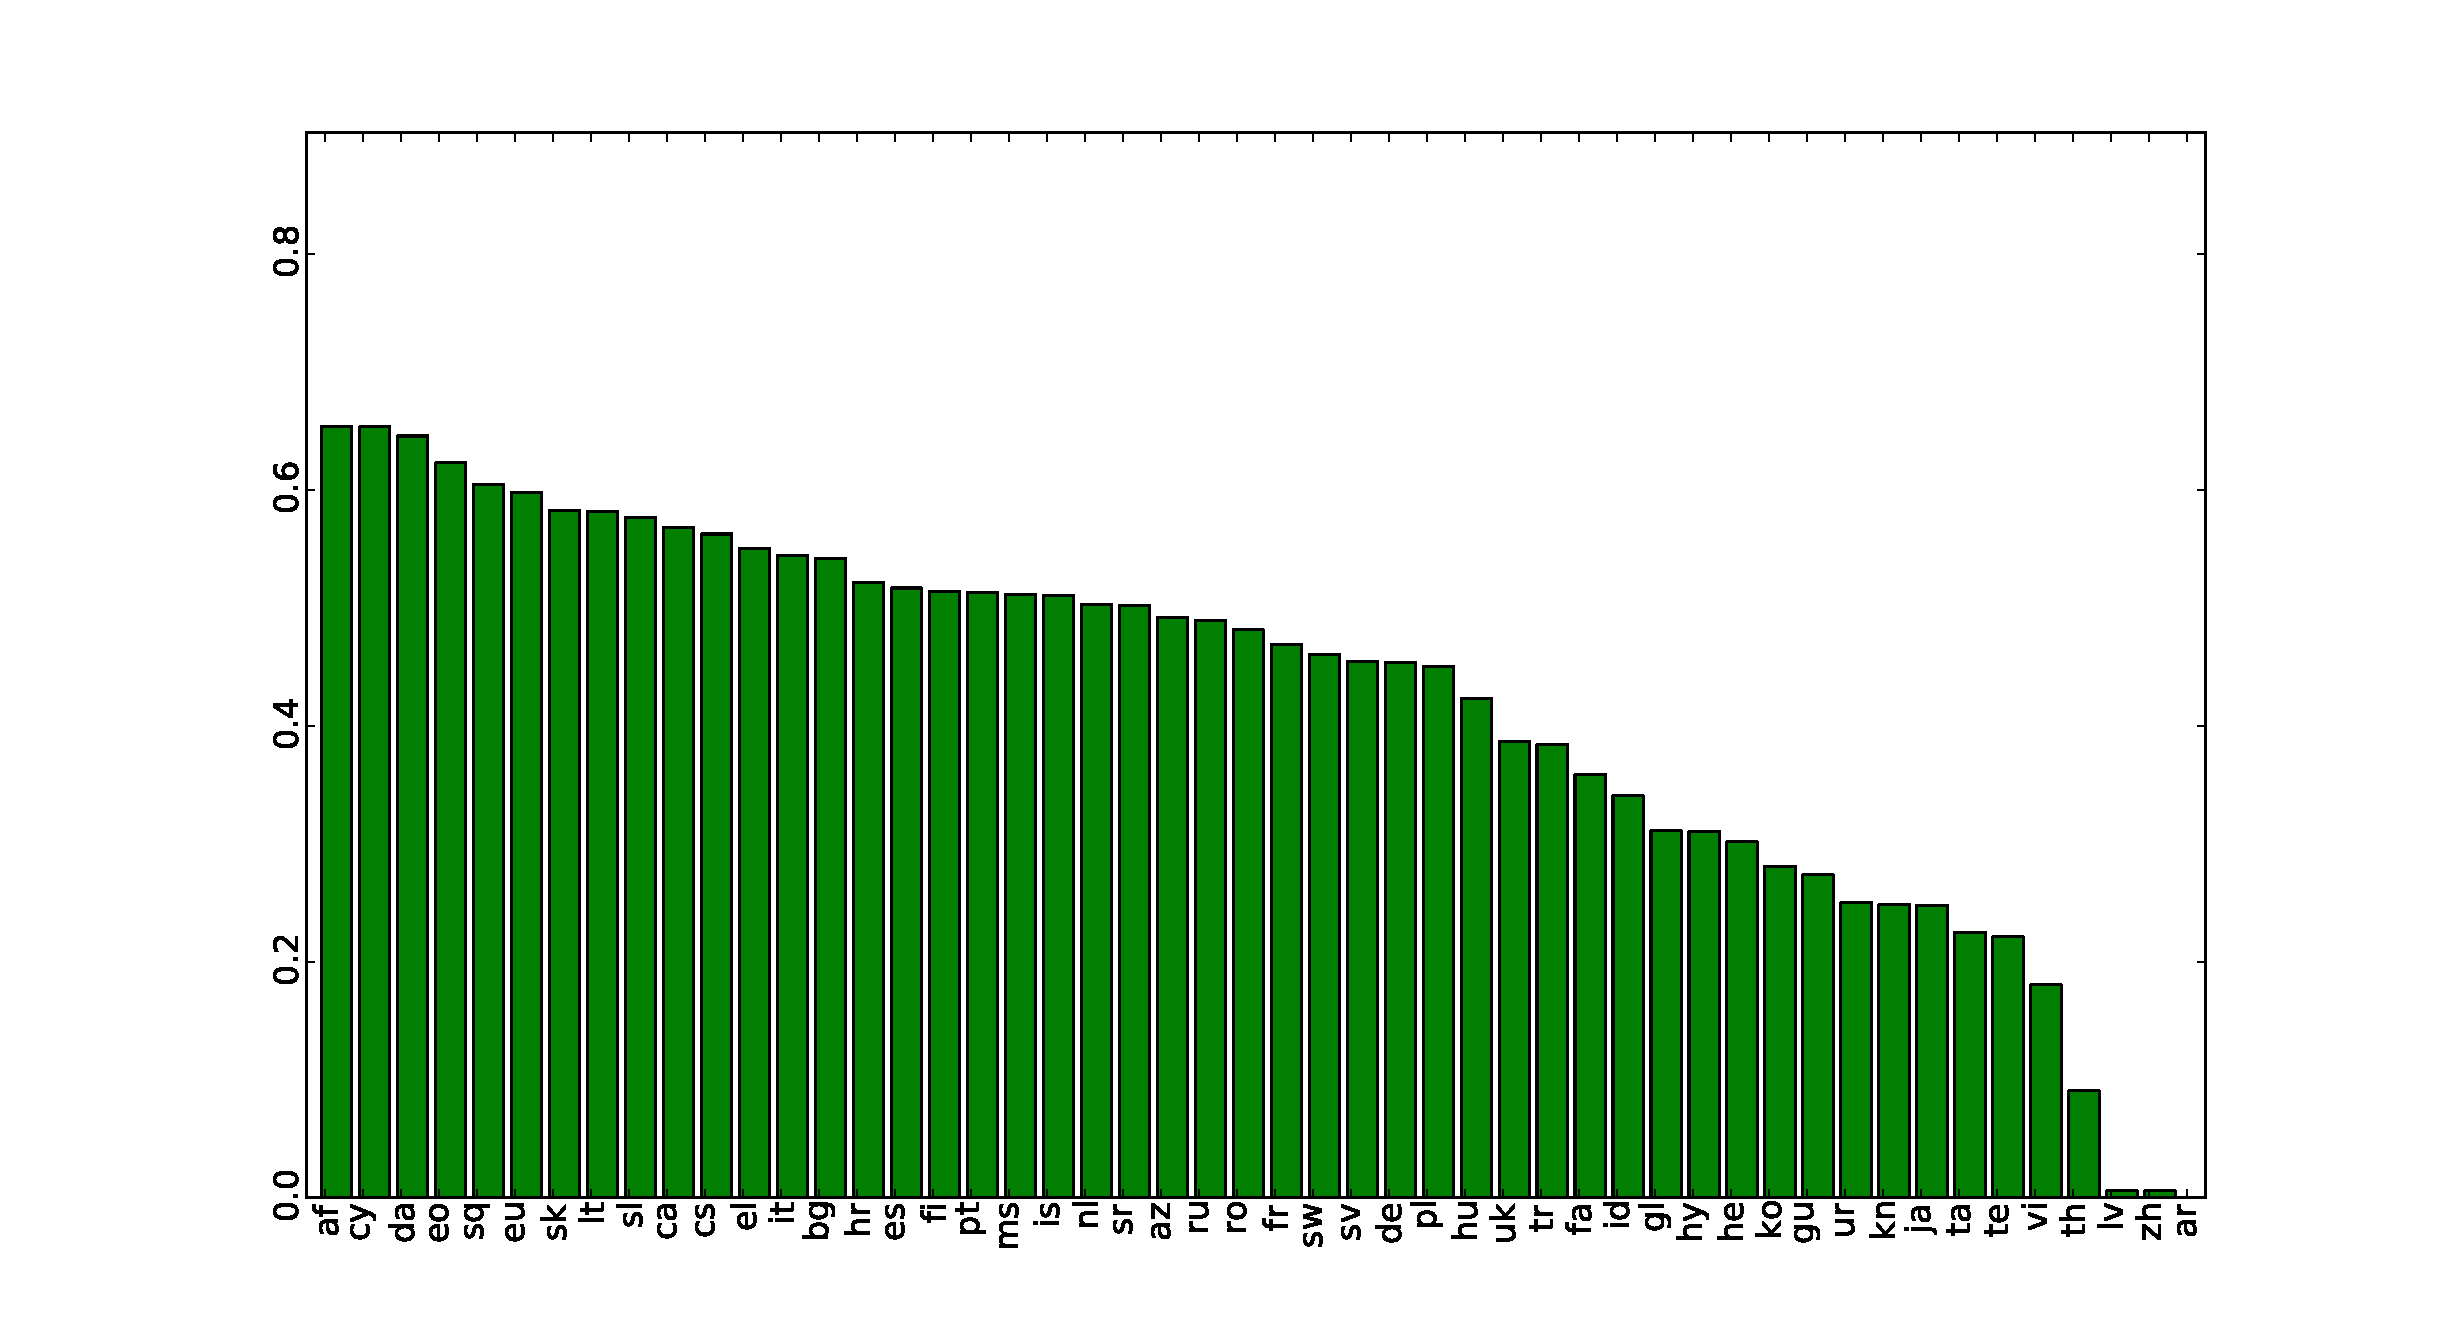
\includegraphics[width=1\linewidth]{final-figures/google-match}
\caption{Average proportion of Turker translations matching GoogleTranslate, per assignment. Overall average overlap was 0.42}
\label{googlematch} 
\end{center}
\end{figure}
%%%%%%%%%%%%%%%%%%%%%%%%%%%%%%%%%%%%%%%%%%%%%%%%%%%%%%%%



%%%%%%%%%%%%%%% QUALITY / NUM ASSIGN SCATTER %%%%%%%%%%%
\begin{figure*}[h]
\begin{center}
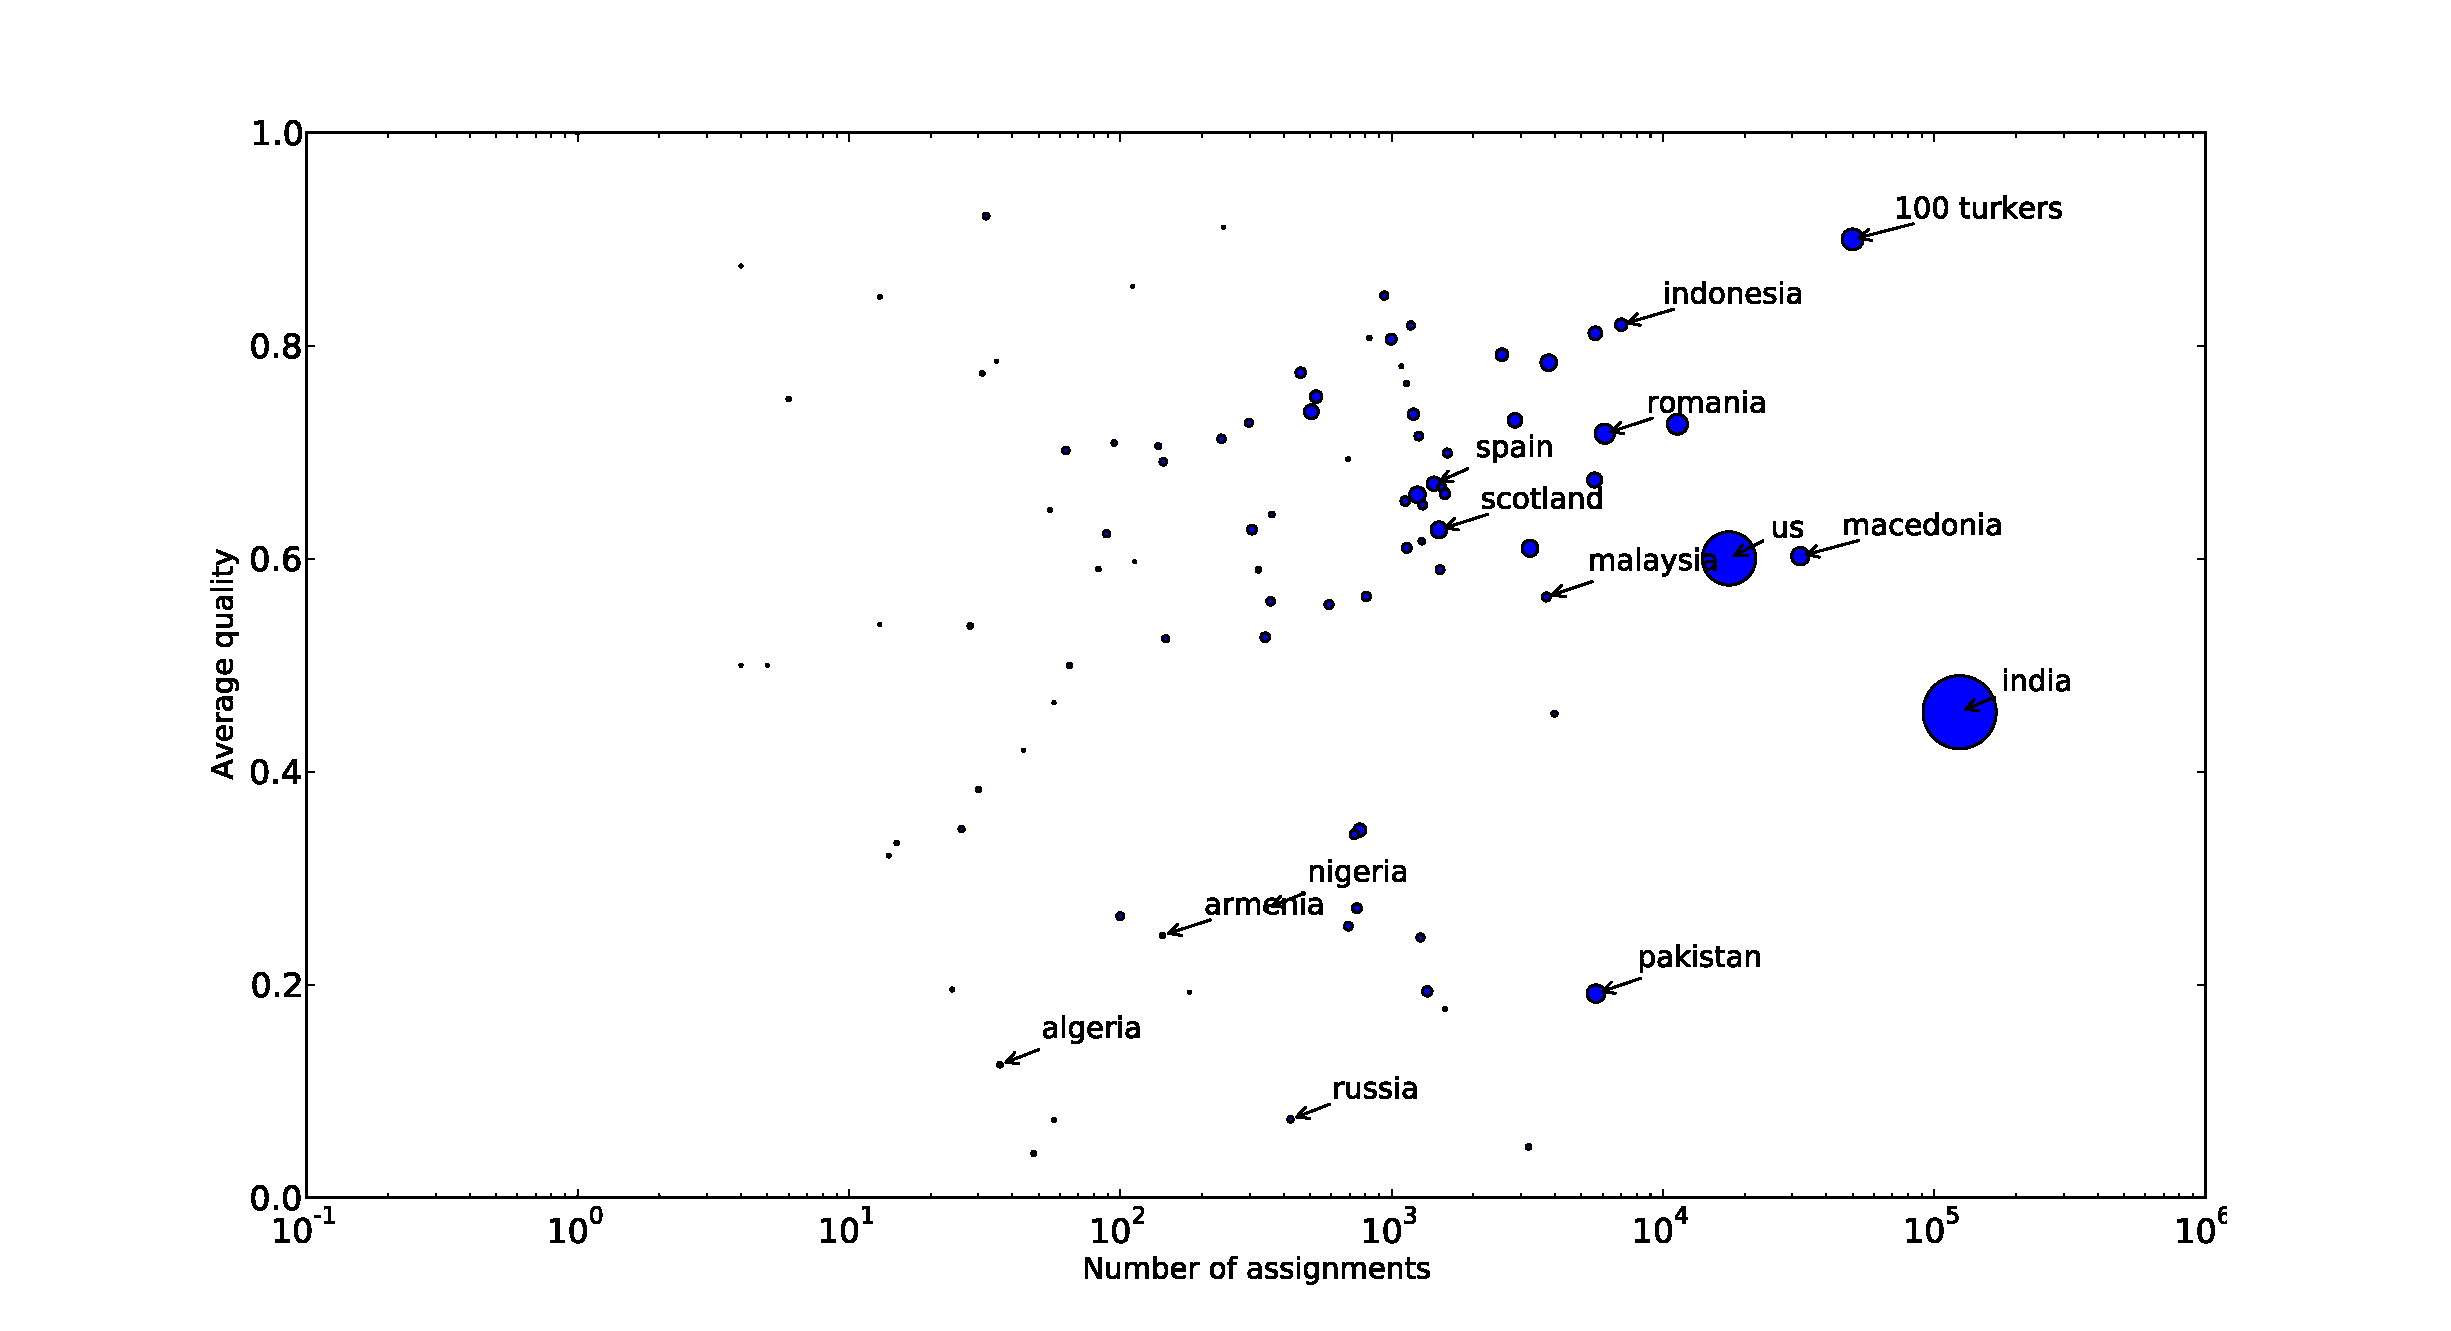
\includegraphics[width=.8\linewidth]{final-figures/quality-scatter}
\end{center}

\caption{Estimated quality of translations by country. Each circle is a country, sized proportional to the number of active Turkers from that country. Quality is calculated as the average number of control words which were correct translations of the source word, where ”correct” means that the provided translation was judged to be synonymous with the known translation by workers in a second-pass HIT. Figure represents data from approx. 295,000 assignments for which geolocation was known.}
\label{quality-scatter}
\end{figure*}
%%%%%%%%%%%%%%%%%%%%%%%%%%%%%%%%%%%%%%%%%%%%%%%%%%%%%%%%

Figure \ref{quality-scatter} shows the number of assignments competed per country and per-country quality estimates.

\paragraph{Use of machine translation}


Given then prevalence of out of region workers, we investigated what proportion of the translations submitted by workers were simply replicating translations from a machine translation system.  Although we followed best practices to deter copying-and-pasting into online MT systems  by  rendering words and sentences as images \cite{zaidan-callisonburch:2011:ACL-HLT2011a}, this strategy does not prevent workers from typing the words into an MT system, if they are able to type in the language's script. 

We used Google Translate to translate all 10,000 words for 50 foreign languages that Google Translate covers. We measured the percent of translations received that exactly matched the translation returned from Google translate. Results are show in Figure \ref{googlematch}. 
Assignments averaged around 42\% overlap with Google translate.  Languages with non-Latin scripts (such as the Arabic script, Chinese characters or the Telugu alphabet) have lower overlap with Google,  suggesting that it is easier for Turkers to cheat for languages written in the Latin alphabet. 
% suggesting that it is easier for Turkers to use MT for Latin alphabet languages. 



%We translated: af ar az bg ca cs cy da de el eo es eu fa fi fr gl gu he hr hu hy id is it ja kn ko lt lv ms nl pl pt ro ru sk sl sq sr sv sw ta te th tr uk ur vi zh

% Google supports:
%Afrikaans
%Albanian
%Arabic
%Belarusian
%Bulgarian
%Catalan
%Chinese
%Chinese
%Croatian
%Czech
%Danish
%Dutch
%English
%Estonian
%Esperanto
%Filipino
%Finnish
%French
%Galician
%German
%Greek
%Hebrew
%Hindi
%Hungarian
%Icelandic
%Indonesian
%Irish
%Italian
%Japanese
%Korean
%Latvian
%Lithuanian
%Macedonian
%Malay
%Maltese
%Norwegian
%Persian
%Polish
%Portuguese
%Romanian
%Russian
%Serbian
%Slovak
%Slovenian
%Spanish
%Swahili
%Swedish
%Thai
%Turkish
%Ukrainian
%Vietnamese
%Welsh
%Yiddish
%Armenian
%Azerbaijani
%Basque
%Georgian
%Gujarati
%Haitian Creole
%Kannada
%Latin
%Lao
%Tamil
%Telugu
%Urdu

\paragraph{Validation of controls} 
Higher overlap with Google translate corresponds slightly to higher quality scores (Pearson $\rho$ = 0.22), suggesting that some control translations have already been indexed by Google. We therefore investigated the validity of our use of Wikipedia inter-language links as gold standard translations.

As an extrinsic measure of translation quality, we measure the proportion of $<${\it word, translation}$>$ pairs received from Mechanical Turk which appear in external dictionaries.  We had external bilingual dictionaries for 27 of the 119 languages examined in this study.\footnote{The bilingual dictionaries were between English and az, bg, bn, bs, cy, es, fa, hi, id, lv, ms, ne, pl, ro, ru, sk, so, sq, sr, ta, tr, uk, ur, and uz. }  We used each of these bilingual dictionaries to computer language-level quality scores, using the dictionary's translation as a gold standard translation for any of the 10,000 foreign words in our study.  In some cases, the overlap of words was low, since dictionaries list root forms of words and we translated inflected forms.  

We ranked the 27 languages based on their translation quality scores according to the external dictionaries, and calculated correlation when compared to the ranking produced by our gold standard control.  The Pearson correlation was $\rho=0.53$.  We computed a correlation coefficient of $\rho=0.37$ for ranking of the translation quality of individual Turkers using the two sources of reference translations.    

Given the strong positive correlation, we are satisfied that the trends reported in this paper hold when using either our gold standard translations or external bilingual dictionaries. 





\section{Discussion}
The Mechanical Turk gives research access to a diverse set of bilingual workers, making it a promising resource for researchers and developers of multilingual systems. 
Although unfiltered data can contain large amounts of noise, 
a variety of techniques can be incorporated into crowdsourcing pipelines to ensure high quality data.  Based on our study, we suggest restricting workers to countries that plausibly speak the foreign language of interest, and embedding gold standard controls where possible, rather than relying solely on self-reported language skills.

Although our study targeted bilingual workers on Mechanical Turk, and neglected monolingual workers, we believe our results reliably represent the current speaker populations, since the vast majority of the work available on the crowdsourced platform is currently English-only.  We therefore assume the number of non-English speakers is small.  In the future, it may be desirable to recruit monolingual foreign workers.  In such cases, we recommend other tests to validate their language abilities in place of our translation test.  These could include performing narrative cloze, or listening to audio files containing speech in different language and identifying their language. 


\section{Data release}

We plan to release all data and code used in this study upon publication of this paper.  Our data release will include the raw data, along with bilingual dictionaries that are filtered to be high quality. It will include 308,079 translation assignments from 5,277 Turkers and 20,955 synonym assignments from 1,006 Turkers, along with meta information like geolocation and time submitted, plus external dictionaries used for validation. The dictionaries will contain 850,907 total translated words in 101 languages, along with code to filter the dictionaries based on different criteria. 
 

\bibliographystyle{acl2012}
\bibliography{mturk}

\end{document}
